\documentclass[thesis.tex]{subfiles}

\begin{document}

\chapter{Prerequisites and Related Work}  \label{chap:preqAndRel}

This chapter lists and describes the necessary topics to follow this thesis. It explains SCION's structure, functionality and details about the component as for example the border router. SCIONLab itself and its work is also outlined. At last, a short description about Prometheus and its used features will be given to understand how the experiment was done.
The second part of the chapter will list related works which tried to solve the problem of multi path communication abuse by regulating or monitoring the behavior. The work on SIPRA and a VirtualCredit system will be presented, which are designed for SCION. Additional work for other types of networks will also be discussed.

\section{Prerequisites} \label{chap:preq}

\subsection{SCION} \cite{SCIONPaper, SCIONBook}

SCION, an acronym for \textbf{S}calability, \textbf{C}ontrol and \textbf{I}solation \textbf{O}n \textbf{N}ext-generation networks, provides a green-field solution for problems of the current Internet, which is named in this content as the \textit{legacy internet}. The main difference between them is \textit{path-transparency}. In the current existing IP routing protocol the end-hosts cannot chose a path, but must rely on the router between them to find a good path. This leads to the problem, that the receiver cannot verify, if the packets were modified nor if the taken path was trustworthy. SCION allows the end hosts to chose between communication paths and also to see the path of a packet on the end-host. The fundamental change needs a different organization of the network nodes, which will be described in this part.

\autoref{fig:prequirement:scionStructure} shows an example SCION network from \cite{SCIONPaper}. This topology consists of \textbf{Is}olation \textbf{D}omains (ISD) and each node of it is considered an \textbf{A}utonomous \textbf{S}ystem (AS). They represent exactly one physical end-host, a whole companies network or an \textbf{I}nternet \textbf{S}ervice \textbf{P}rovider (ISP)'s network. Each ISD is administered and initially created by a small group of ASes, which are referred to \textit{Core} ASes and forms the \textit{Core} of an ISD. They are responsible to define a policy which applies to all member of the ISD and is called the \textbf{T}rust \textbf{R}oot \textbf{C}onfiguration (TRC). Concluding this each ISD has its own rules to create connection and also defines the name the ISD. The Core ASes are also connect with other ISDs and link their ISDs to them. Additionally an AS can belong to multiple ISDs at one time, which is the case for the AS \textbf{H}.



\begin{figure}[h]
	\centering
	\begin{subfigure}{.48\linewidth}
		\centering
		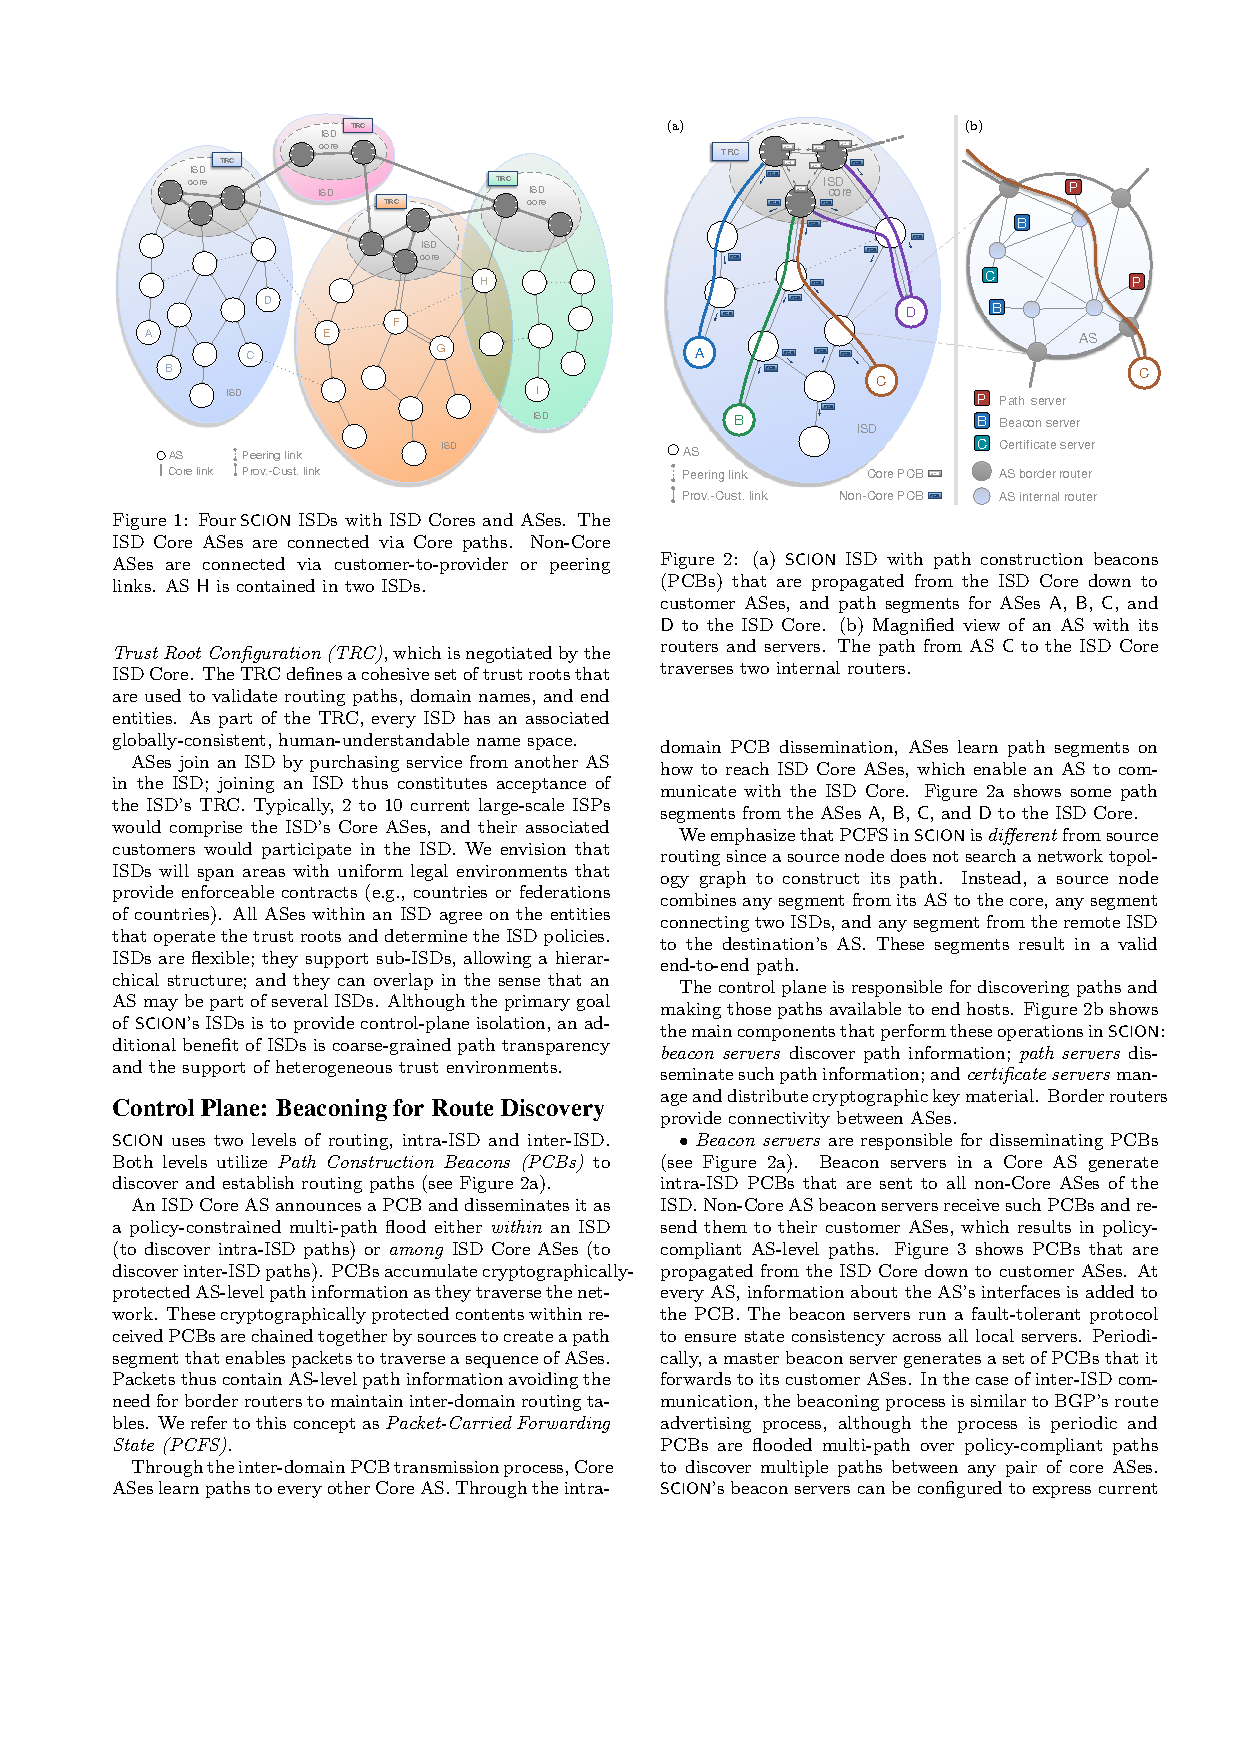
\includegraphics[trim=19mm 214mm 105mm 19mm ,clip,height=0.28\textheight]{2015-SCION-short_3.pdf}
		\caption{Four SCION ISDs with ISD Cores and ASes \cite[Figure~1]{SCIONPaper}}
		\label{fig:prequirement:scionStructure}
	\end{subfigure}
	\hfill
	\begin{subfigure}{0.48\linewidth}
		\centering
		\begin{tikzpicture}
		\node[anchor=south west,inner sep=0] at (0,0) {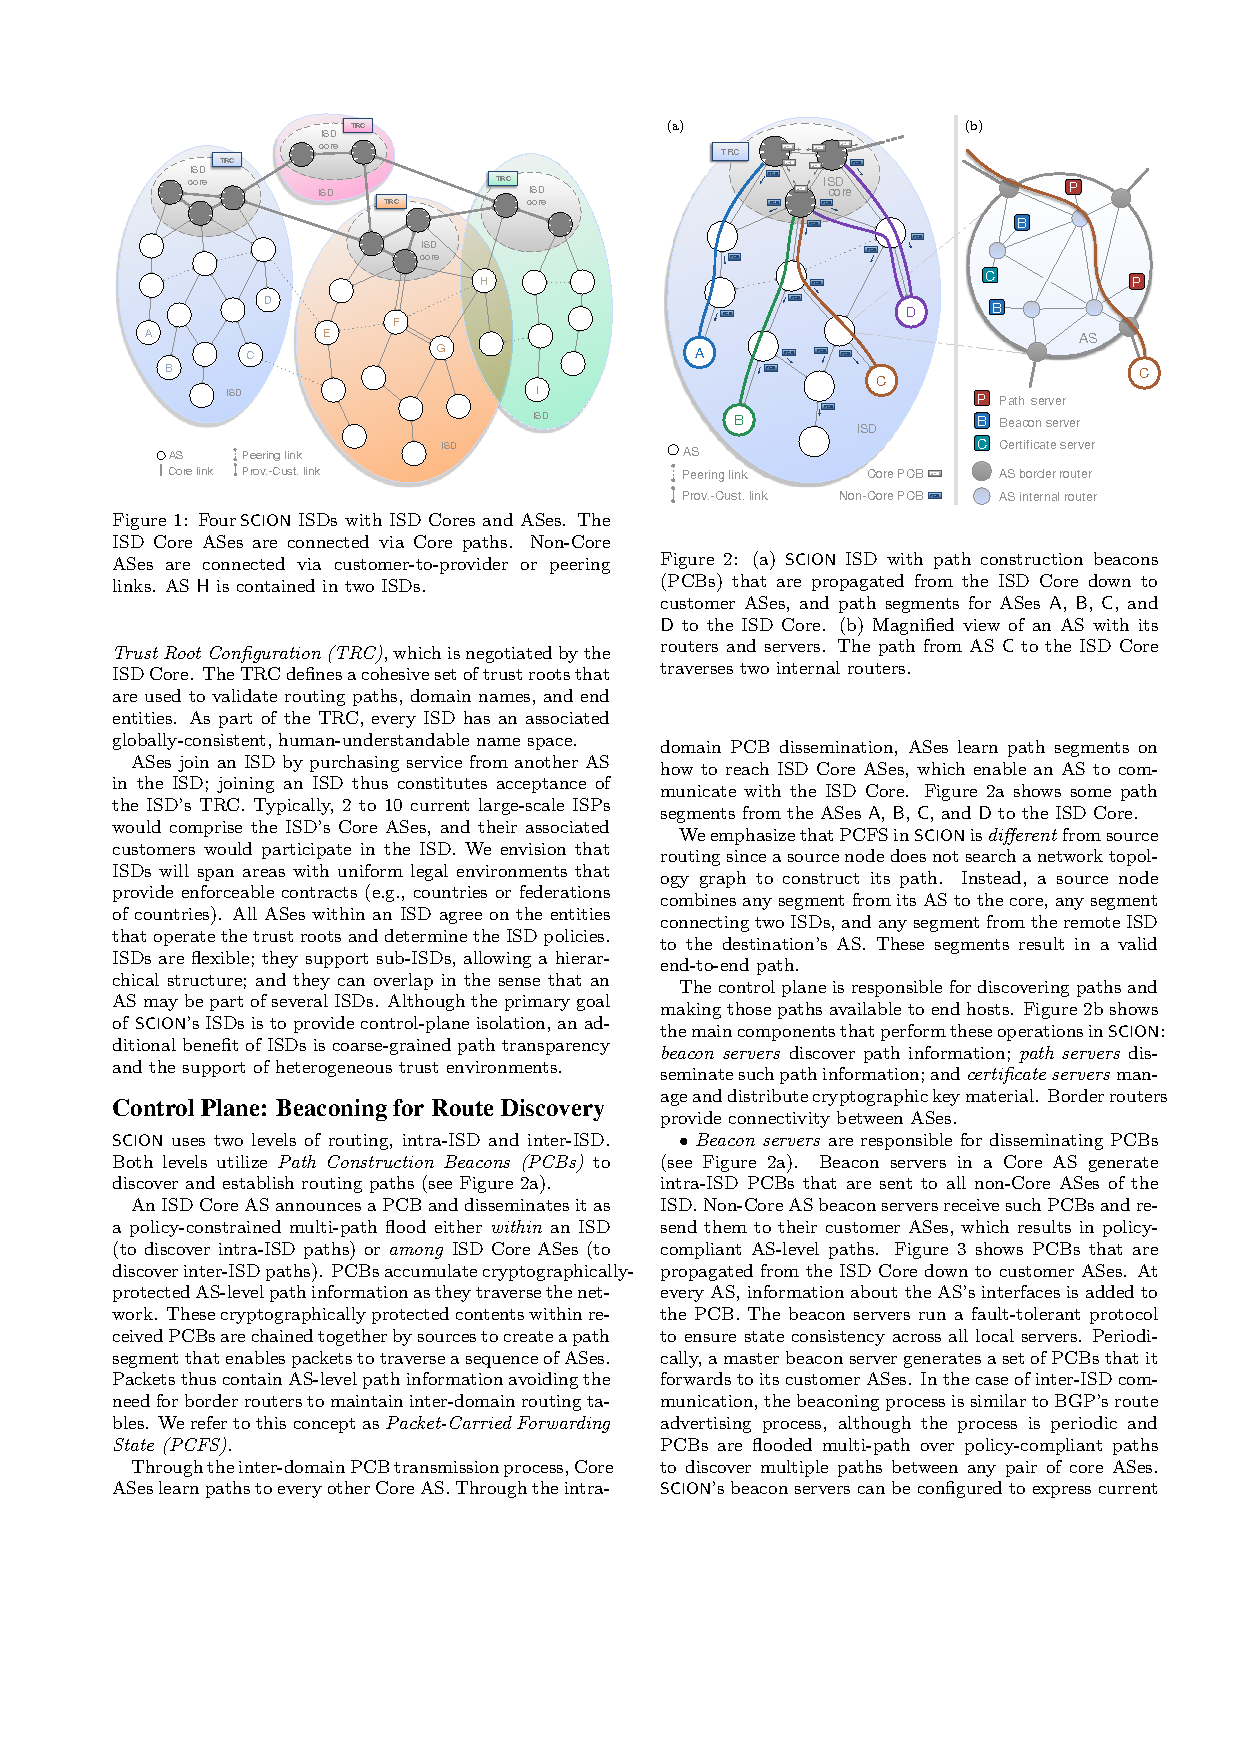
\includegraphics[trim=163mm 210mm 13mm 24mm ,clip,height=0.28\textheight]{2015-SCION-short_3.pdf}};
		\fill[white,rotate=-7] (-0.5,3) rectangle (0.70,3.15);
		\fill[white,rotate=37] (3.2,4.22) rectangle (3.7,4.35);
		\end{tikzpicture}
		\caption{Magnified view of an AS with its routers and servers \cite[Figure~2b]{SCIONPaper}}
		\label{fig:prequirement:AsStructure}
	\end{subfigure}
	\caption{Structure of SCION with an example topology.}
	\label{fig:prequirement:structureOfScion}
\end{figure}

Inside an AS (see \autoref{fig:prequirement:AsStructure}) exists multiple router to route the traffic from one link to another. Each link is administered by one \textit{border router}, while the \textit{internal router} forward the packets inside the AS itself.

An AS needs to know the path to another AS to communicate to them. This routing problem is solved with a process called \textit{beaconing}. A core AS announces such a beaconing inside its ISDs and learns the different paths from a core AS to a non-core AS. The ASes respond to this beaconing and over time the topology is created. On the other side, a non-core AS explores by beaconing the paths to the core-AS. The same procedure is done for inter-ISD communication by the core-ASes. The up-segment from a non-core AS to the Core and the down-segment from the beaconing of a core-AS are merged together and send to the \textit{path-server}. This component handles routing requests from one AS to another AS and responds with a set of possible paths to take. The elements of this set depend on the TRC of the ISD. For example, one ISD does not want to enable multiple path communication and only responds with the first available path.

One advantage of this structured routing is that a communication does not leave an ISD when it is not necessary. This enables to create ISDs for different security or efficiency scenarios. Packets are only routed in a trusted zone when they need to be. The legacy internet do not guarantee this behavior. A packet from OvGU-Magdeburg to ETH-Zuerich could be routed over different location in the world without control over it. If both of them were inside one ISD containing only research institutes, than the packet would be guaranteed to not leave this ISD because it is not necessary.

Another advantage is the possibility to choose an alternative way. This is interesting in cases a path segment has a failure and should be avoided for different reasons like malicious attacks or technical failures. The legacy internet relies on the Border-Gateway-Protocol (BGP) \cite{rekhter2005border, Halabi.1997}, when was inspected by many researcher for its fault-tolerance and stability. It was also shown in \cite{Sahoo.2006} that the reaction time (convergence) for realistic topologies takes seconds to minutes for the protocol to adjust to failures. A similar result was given by \cite{Labovitz.2001} of a delay of 3 minutes for 30\% the cases and even higher as 15 minutes in total. In SCION this slow reaction problem is minimized by letting the user choose different path. If one path is not responding the node can request for another path or use one of the provided alternatives.

The multiple paths to the target can also be used for a better bandwidth utilization. Instead of sending the data over only one link the stream can be split into multiple sub streams and transfered over the available paths to the target. 
This leads to a better utilized networks capacity because otherwise unused links are used and not idle. Bandwidth is cannot be saved or stored, it can only be used in a moment or it would be wasted. But this also can lead to an unwanted flood of the network and can create multiple congestions, unintentionally. This would negate the advantage and should only be used with caution. Because of the potential misuse of such a multipath communication several studies have been conducted which are explained in \autoref{chap:prevwork}

The legacy internet cannot be replaced at once but can only be updated or replaced incrementally. This process can take many years as seen for the deployment of IPv6. The update for a necessary address space expansion was firstly published in 1998\cite{Deering.1998} and its adoption rate is in 2018 only at around 22\% \cite{GoogleInc.} to 24\% \cite{Ripenetworkcoordinationcentre.18.04.2018}, even the IPv4 address space ran out on 03.02.2011\cite{ICANN.03.02.2011}. Similar to the transition from IPv4 to IPv6 there is a need for a transition from the legacy internet to SCION, which is realized with the \textbf{S}CION-\textbf{I}P \textbf{G}ateway. It encapsulates the IP packets in SCION packets to interact with the legacy internet.

This description is only an overview about the complexity and mechanism of SCION, but this will be sufficient to understand the nature of this work. For further reading it is recommended to start with the paper of Adrian et. al\cite{SCIONPaper} and go into details with the published book of Adrian et. al\cite{SCIONBook}.



\subsection{SCIONLab}

SCIONLab\footnote{\url{https://www.scionlab.org}, 18.04.2018} is the test environment to test out SCION and its functionality in a running network. Its current topology can be seen in \autoref{fig:prequirement:scionlabTopo}. Any interested user is able to create an AS as a VM which is automatically configured and ready to deploy. They can choose different attachment points their AS is creating a connection to. This system enables user to simply test out SCION in a sandbox without additional impact.

\begin{figure}
	\centering
	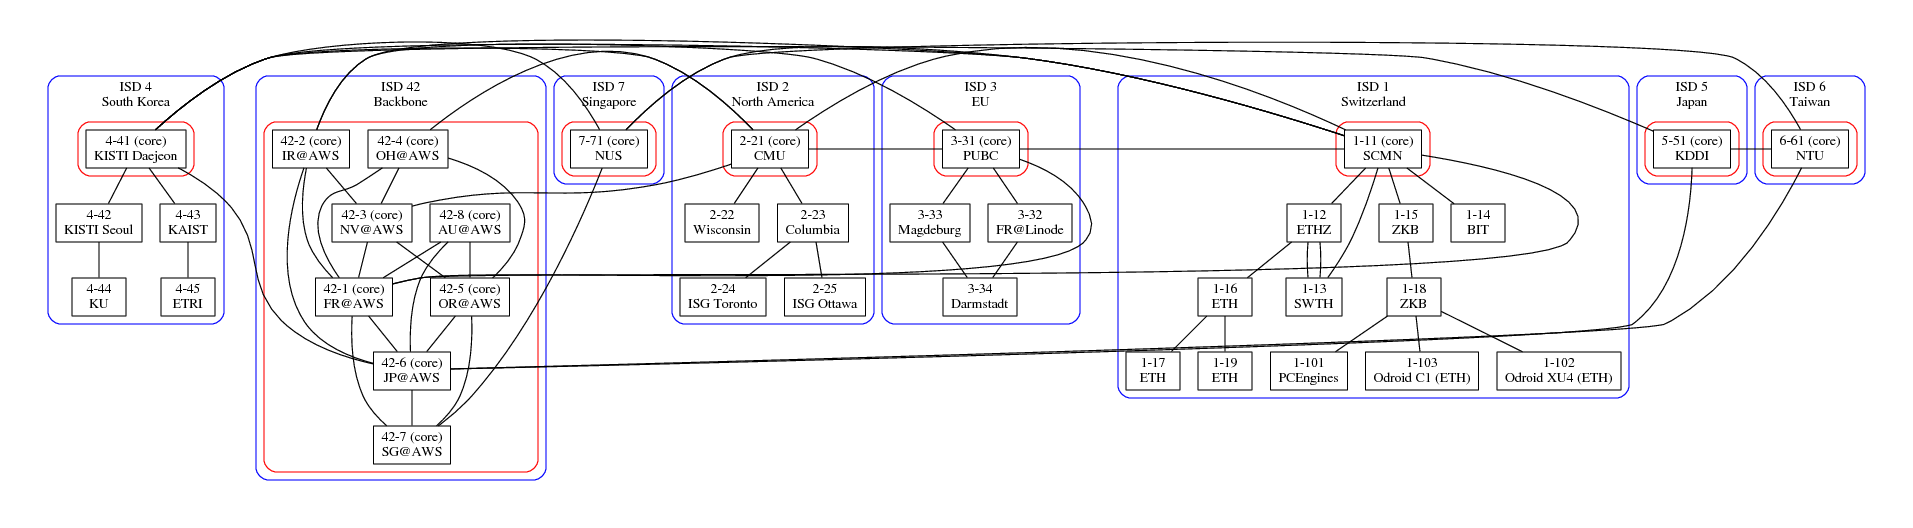
\includegraphics[width=0.95\linewidth]{topology_no_labels.png}
	\caption*{\tiny{\url{https://www.scionlab.org/public/img/topology_no_labels.gv.png} (18.04.2018)}}
	\caption{SCIONLab topology. Shows the major ASes without the user VM. The core ASes are bordered in red}
	\label{fig:prequirement:scionlabTopo}
\end{figure}

\subsection{Prometheus} 

"Prometheus is an open-source systems monitoring and alerting toolkit [...]" \footnote{\url{https://prometheus.io/}, 18.04.2018}. This framework consisting of a \textit{Prometheus server} and an API to create and gather data about programs, which is implemented by the \textit{Prometheus clients}. Each client defines a data model of different \textit{metrics} to monitor. These metrics are collected by the Prometheus server in a given scrap interval and stored on the server side. A simple Web UI enables the user to write queries and analyze the data, for example extracting the maximum bandwidth at a given time.

The client API defines four different metric types. The \textit{counter} represents a data which can only go up while the \textit{gauge} can also go down over time. An example for a counter is the total bandwidth in bytes since the border router start while a gauge can be the current memory usage. The two other types are the \textit{histogram}, which samples observations in different buckets, and the \textit{summary} which does the same as a counter but also calculates quantiles over a sliding time window. Each metric consists of the value itself as a double-precision floating point number and a UTC time stamp. The client defines the type of the metric and the name and continually updates the value. The metrics are exported over an HTTP based API. The endpoint is typically {\lstinline|http://[HOST]:[PORT]/metrics|} which responds with a list of all metrics and their values at the time of request. The Prometheus client API was already implemented in the border router, the path, the beaconing and the certificate server. An example of this is seen in \autoref{app:promMetric}

\section{Related Work}\label{chap:prevwork}

This section will list and describe work by other people with similar problems or thoughts. It will show their difference to this work and why this work exists.

\subsection{SIBRA} \label{sec:prevwork:sibra}

The \textbf{S}calable \textbf{I}nternet \textbf{B}andwidth \textbf{R}eservation \textbf{A}rchitecture (SIBRA) is an approach against resource overuse by Basescu et. al \cite{Basescu.2016}. The architecture enables nodes to reserve a certain bandwidth for a time slot. This bandwidth is guaranteed for the flow and is not shared with other user on the path. The main reason to establish such a system were the increasing DDoS attacks and the flaws of the defenses against it. Over the last years the amount and size of DDoS attacks are increasing as shown in the life visualization \cite{GoogleInc.2013}. The largest recorded DDoS occurred on the 28th of February in 2018 on github.com with a peak of 1.35Tbps \cite{Kottler.01.03.2018}. SIBRA invented a mechanism that two nodes can communicate with each other even in the presence of malicious nodes disturbing the network.

This was achieved by introducing three layers of contracts for a guaranteed bandwidth. Each of them differ in time and dimension: The \textbf{core} are \textit{long-term} contracts and are established between the core ASes of different ISDs. Within an ISD the ASes conclude contracts intermediate-term with each other which are called \textbf{steady}. They are used for a steady, but low bandwidth transition. A \textit{short-term} contract, called \textbf{ephemeral}, is conducted between two end-hosts. These are reserved for high bandwidth traffic. 

A link's capacity is divided into three partition: 80\% is reserved for ephemeral path, 5\% for steady paths, and 15\% are for best-effort. An ephemeral path is created by sending a request through a steady path and contains the amount of bandwidth to reserve and a time slot to use. The default life time of such a path is 16 seconds and the time slot granularity is 4 seconds. A packet using a SIBRA reservation contains a flow ID, an expiration time, a bandwidth class, a path direction type and a reservation index. The SIBRA router maintain a \textit{bandwidth table} to store the reserved bandwidths of the router's neighbor, an accounting table to keep track of flow ids and their attributes, and a \textit{pending table} for pending reservation. A SIBRA packet with an invalid header will use the best-effort bandwidth.

This enables SIBRA to efficiently control malicious flows. A botnet AS can be excluded from reserving bandwidth and the best-effort band is never disturbed. That mechanic solves the problems of this work and were already established and tested in SCION. The reason for this work is that SIBRA is very complex to implement and not suitable for SCIONLab's test environment. A simpler approach was needed to identify malicious user or prevent them.

\subsection{Virtual Credit} \cite{Meyer.2017}
Another approach to reserve bandwidth and limit the abilities of malicious user was introduced by Meyer et. al for SCION. The base idea was that an AS can only use resources when it also provide them to the network. This was realized by introducing a \textit{virtual credit} an AS can use to buy capacity. It would only gain such a credit if it provides capacity. The intention was to motivate user not only use the networks resource but also provide them by establishing new connection or building new infrastructure elements like fiber cables or backbones.

It was based on the monitoring system RIPE Atlas \cite{Ripenetworkcoordinationcentre.19.04.2018} which enables user to monitor traffic and send probe requests. To do so they need credits which they gain when they provide a usable probe.

One virtual credit is worth 10 MBits/s of capacity to reserve without an expiration. When one AS requests such a connection to another AS, the second AS would get the credit the requester invested. Each AS starts with 100 credits which is worth of 1 GBit/s. This simple design prevents AS to use more bandwidth than they would provide. A malicious user would need other ASes to establish connection to it to gain credit and use it for a malicious attack.

This alternative approach to prevent an overuse was not considered because it was easily exploitable as shown in the paper itself. A malicious AS can spawn multiple virtual ASes which connects to the malicious AS. This one now has the credits of the virtual ASes but they do not improve network. The malicious AS can use their credits to flood the network. Because of this exploits in such a basic concept it was not considered for this work.

\subsection{Delay-Tolerant Networks}
Zhu et. al \cite{Zhu.2014} created a system called \textit{iTrust} to detect nodes in a delay-tolerant network which does not honestly forward messages. The forwarding of messages is important in such network as they suffer from frequent disconnection. Examples of them are sensor networks with a temporary connection to each other or mesh networks on smartphones. A malicious node could drop messages instead of forwarding them as intended. Zhu et. al use the inspection game to calculate the probability to inspect a single node if it acts suspicious. They showed that using this model can reduce the detection overhead. The idea of using Game Theory to model such a system was used in this work.

\subsection{Inspection Game in other contexts}
The \textit{Inspection Game}, part of the \textit{Game Theory}, is used in this work as a theoretical model for the monitoring. While described later in detail, the inspiration for this were from other applications. They are examples that the Inspection Game is a general construct with many application, even outside the topic of networking. Nozenzo et. al \cite{Nosenzo.2014} examined the effectiveness of this model in regards to bonus for comply and a fine for not. They showed that the existence of such a fine improves the behavior of the players but that a bonus has a low impact. 

Avenhaus et. al \cite{Avenhaus.1996} showed the application of this game model for the nuclear arms control from the years 1961 to the present 1996. They described the cost of an inspection and that a constant inspection is not realizable because of limited resources. Also a real world application for it was done by Kirstein \cite{RolandKirstein.2009} to show the effects for doping in sport.

\subfilebib % Makes bibliography available when compiling as subfile
\end{document}